\documentclass{beamer}
\mode<presentation>{\usetheme{boxes}\setbeamercovered{transparent}}
\usepackage{graphics, graphicx, hyperref}
\renewcommand{\vec}[1]{\mathbf{#1}}
\graphicspath{{../graphics/}{../drawings/}}
\beamertemplatenavigationsymbolsempty
\addtobeamertemplate{block begin}{\setlength\abovedisplayskip{0pt}}

\title{Transient Effects in the Optical Pumping of Rubidium}
\author{Giacomo Resta}

\begin{document}
\frame{\titlepage}

\frame{\frametitle{Transient Effects}
\begin{itemize}
\item Measurements of re-population rate with varying, 
\begin{itemize}
\item Light Intensity
\item Vapor Temperature
\item Magnetic Field Tangent to Optical Axis
\item Magnetic Field Along Optical Axis 
\end{itemize}
\item Measurements of Rabi oscillation period with varying,
\begin{itemize}
\item RF Amplitude
\item RF Frequency
\end{itemize}
\end{itemize}
}

\frame{\frametitle{Energy Structure of Hydrogen-Like Atoms in a Magnetic Field $B_z$}
\begin{figure}
\includegraphics[width=1.0\linewidth]{h_structure.png}
\end{figure}
%\[H = H(l) + I\cdotJ-\frac{\mu_j}{J} J \cdot B - \frac{\mu_I}{I} I \cdot B\] 
}

\frame{\frametitle{Photon Induced Energy Transitions in a Magnetic Field}
\begin{block}{Circularly-Polarized Light}
\begin{align*}
\text{Right-Handed} &\rightarrow\vec{\sigma^+} \\
\text{Left-Handed} &\rightarrow\vec{\sigma^-}
\end{align*}
\end{block}
\begin{block}{$\Delta M_z = +1$}
\begin{align*}
\vec{B_z} \cdot \vec{\sigma^{+}} &> 0 & \Delta M_z = +1\\
\vec{B_z} \cdot \vec{\sigma^{-}} &< 0 & \Delta M_z = +1
\end{align*}
\end{block}
\begin{block}{$\Delta M_z = -1$}
\begin{align*}
\vec{B_z} \cdot \vec{\sigma^{+}} &< 0 & \Delta M_z = -1\\
\vec{B_z} \cdot \vec{\sigma^{-}} &> 0 & \Delta M_z = -1
\end{align*}
\end{block}
}
\frame{\frametitle{Optical Pumping of Hydrogen}
Right-Handed Circularly Polarized Light
\begin{align*}
\vec{B_z} \cdot \vec{\sigma^+} > 0  && \Delta M_z = +1
\end{align*}

\begin{figure}
\includegraphics[width=1.0\linewidth]{h_pump_up.png}
\end{figure}
}

\frame{\frametitle{Optical Pumping of Hydrogen Following $B_z$ Reversal}
Right-Handed Circularly Polarized Light
\begin{align*}
\vec{B_z} \cdot \vec{\sigma^+} < 0  && \Delta M_z = -1
\end{align*}

\begin{figure}
\includegraphics[width=1.0\linewidth]{h_pump_down.png}
\end{figure}
}

\frame{\frametitle{Experiment Apparatus}
\begin{figure}
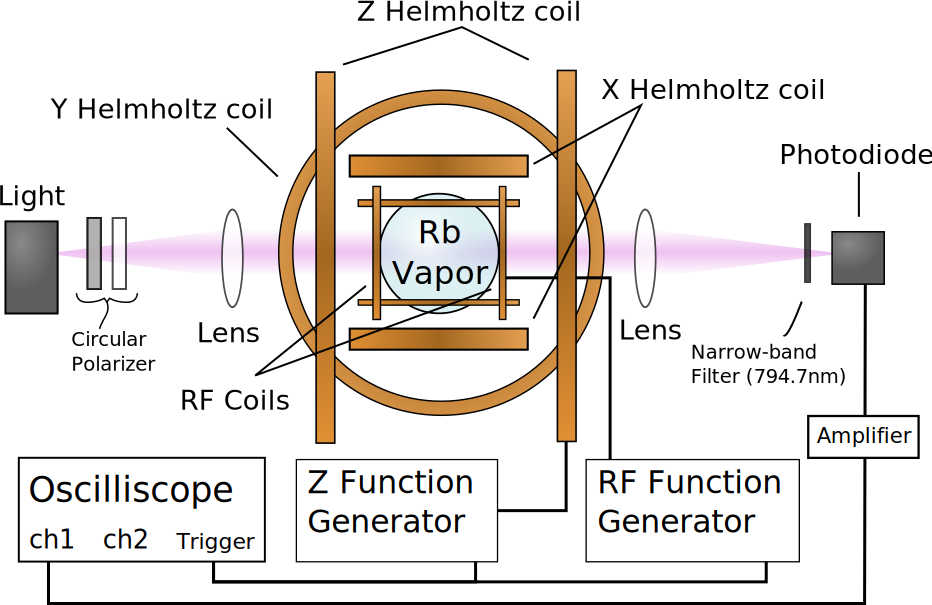
\includegraphics[width=1.0\linewidth]{setup.png}
\end{figure}
}

\frame{\frametitle{Photo-diode Voltage With $B_z$ Current}
\begin{figure}
\includegraphics[width=1.0\linewidth]{wf_overview.png}
\end{figure}
}

\frame{\frametitle{Simulation of Optical Pumping of Atomic Models with Different Numbers of $M_z$ Levels}
\begin{figure}
\includegraphics[width=0.9\linewidth]{theory_wf_fit.png}
\end{figure}
}

\frame{\frametitle{Towards a Functional Approximation for Rubidium Signal}
Assuming a Hydrogen like, three $M_z$ level structure,
\begin{align*}
\frac{dn_1}{dt}&=n_0a_0\\
\frac{dn_0}{dt}&=-n_0 a_0 + n_{-1} a_{-1}\\
\frac{dn_{-1}}{dt}&=-n_{-1} a_{-1}
\intertext{hence,}
\frac{d^2n_0}{dt^2}&=-(a_{-1}+a_{0})\frac{dn_0}{dt}-a_{-1}a_{0}n_0
\intertext{Assuming $a_{-1} = a_{0}$,}
I(x) &= c_4-c_0(t+c_1)\exp\left({-c_2(t-c_3)}\right)
\end{align*}
}

\frame{\frametitle{Rabi Oscillations Signal Overview}
\begin{figure}
\includegraphics[width=1.0\linewidth]{rabi_overview.png}
\end{figure}
}

\frame{\frametitle{Rabi Oscillation Period vs RF Amplitude}
\begin{figure}
\includegraphics[width=1.0\linewidth]{rabi_fit.png}
\end{figure}
}

\frame{}
\end{document}
